\documentclass[a4paper]{article}
\usepackage{amsmath}
\usepackage{amssymb}
\usepackage{geometry}
\usepackage{natbib}
\usepackage{float}%稳定图片位置
\usepackage{graphicx,subfig}%画图
\usepackage{caption}
\usepackage[english]{babel}
\usepackage{indentfirst}%缩进
\usepackage{enumerate}%加序号
\usepackage{multirow}%合并行
\usepackage{hyperref}
\usepackage{verbatim}
\usepackage{geometry}%设置页边距
\geometry{top=1in,bottom=1in,left=1in,right=1in}
\begin{document}
\begin{center}
    \Large{\textbf{SI618 Exploratory Project Report}}\\
    \large{Chongdan Pan $\bullet$ pandapcd $\bullet$ pandapcd@umich.edu}
\end{center}
\section{Summary and Motivation}
Recently, cryptocurrencies like Bitcoins have become the hottest topic all over the world. Cryptocurrencies are being used in multiple areas including decentralized finance, application development, art collections, etc. The market value also increased dramatically in the past 10 years, from less than one hundred dollars to more than two trillion dollars.

\par However, cryptocurrencies are not only about price. Some people are complaining that Bitcoins are wasting more and more energy for meaningless purposes while others are amazed by its decentralized transaction. Therefore, this project will perform a time series analysis, to investigate these ideas and try to find the relation between cryptocurrencies' users, miners, transactions, and price.

\par In details, this project will focus on three main problems
\begin{enumerate}[1]
    \item Does Bitcoin work as it is supposed to?
        \begin{enumerate}
            \item Does it do a good job at controlling the network difficulty and block production rate?
            \item Can Bitcoin provide a transaction mechanism with a low and stable cost?
        \end{enumerate}
    \item How are people's activities on Bitcoin's blockchain?
        \begin{enumerate}
            \item How many users are using Bitcoin every day?
            \item How many transactions happen every day? Is there any pattern?
            \item How is miners' revenue affected by the blockchain network?
        \end{enumerate}
    \item Can we make profits through cryptocurrencies investment?
        \begin{enumerate}
            \item What's the relation between Bitcoin's price and other activity at exchange or blockchain?
            \item Is Bitcoin the best crypto asset for investment?
        \end{enumerate}
\end{enumerate}

\section{Dataset}
\begin{itemize}
    \item Binance has a lot of public REST API providing cryptocurrencies' historical market data of different frequencies at different times \href{https://binance-docs.github.io/apidocs/spot/en/#market-d\\ata-endpoints}{(https://binance-docs.github.io/apidocs/spot/en/\#market-data-endpoints)}. The data are well-structured and will be used at a daily frequency. For simplicity, only the following three fields will be used.
    \begin{itemize}
        \item \textbf{Close:} The close price in USD of cryptocurrencies everyday at Binance.
        \item \textbf{TradeVolume:} The total trade volume of cryptocurrencies everyday at Binance.
        \item \textbf{TradeCount:} The total trade count of cryptocurrencies everyday at Binance.
    \end{itemize}
    The data's time period is from 2018/11/11 to 2021/11/08, and 1409 tuples are retrieved.

    \item \href{https://www.blockchain.com/charts/difficulty}Blockchain.com provides a lot of statistical data about BTC, especially about its blockchain and the networking \href{https://www.blockchain.com/charts/n-unique-addresses}{(https://www.blockchain.com/charts/n-unique-addresses)}. The data will be used at a daily frequency and with follow fields:
    \begin{itemize}
        \item \textbf{Unique Address: } Every user needs a unique address to receive a BTC. The number of unique address can reflect the attitude of BTC's true believers.
        \item \textbf{Miners Revenue: } Miners are people who use their computers to guess the nounce number of a block. The miner who first get the nounce, will be rewarded with some cryptocurrencies. Miners can sell the cryptocurrencies for revenue.
        \item \textbf{Total Hast Rate:} Mining hash rate is a key security metric. The more hashing power in the network, the greater its security and its overall resistance to attack. Miners are performing hashing to to guess whether the nounce is correct
        \item \textbf{Difficulty: }The difficult is measured by the times of hash rate. Difficulty is adjusted every 2016 blocks (every 2 weeks approximately) so that the average time between each block remains 10 minutes.
        \item \textbf{Total Market Value: } The total market value of BTC in USD, it's calculated by the product of price and the total amount of BTC.
        \item \textbf{Transaction Fee: } Different from exchange, the transaction of blockchain is changing due to the number of miners and transactions.
        \item \textbf{Transactions: } The transaction happens on the blockchain. Some transaction are made through blockchain while others are through exchange. However, it's only those with blockchain really transfer the cryptocurrencies to one address from another.
    \end{itemize}
    The data's time period is from 2018/01/01 to 2021/11/08, and 1095 tuples are retrieved.
\end{itemize}
\section{Method}
\subsection{Question 1}
\subsubsection{How did you manipulate the data to prepare it for analysis?}
    According to the definition of network difficulty and total hash rate, the production time of each block should be their ratio. Therefore, I join these two tables on timestamp and divide the network difficulty by the total hash rate. To make a deep quantitative analysis about the production rate, I also calculate the average and standard deviation of the production time and visualize them with a band. Then I calculate the distribution of production time to get a more detailed evaluation of the blockchain's ability of difficulty adjustment. To calculate the transaction fee, I divide the total transaction fee by the number of transactions each day and try to deseasonalize it. 
\subsubsection{How did you handle missing, incomplete, or noisy data?}
    The data from blockchain.com doesn't cover every day in the period, and each field may cover a different timestamp. After the outer join, I fill up the missing value by the last valid value because future information should never be used.
\subsubsection{What challenges did you encounter and how did you solve them?}
    Although the definition of network difficulty and total hash rate is very clear, the data's units are quite confusing. For network difficulty, the unit is \emph{t} while the total hash rate is \emph{mTH/s}. After simple division, the average production time is around 139710, which is ridiculously wrong because, according to Bitcoin's white paper, the average production time should be around 600 seconds. After reading more articles about the definition of TH/s and t, I figured out that the time should be calculated as 
    $$\text{Production Time(s)}=2^{32}\cdot\text{Network Difficulty(t)}/(10^{12}\cdot\text{Total Hash Rate(mTH/s)})$$
\subsection{Question 2}
\subsubsection{How did you manipulate the data to prepare it for analysis?}
    First of all, I joined the average transaction fee, the number of transactions, close price, unique address, and the miner revenue together on timestamp. To calculate the return of each miner, I divide the total miner revenue by the total hash rate. Since the data are of different units, I used Z-score to normalize them and calculate the correlation matrix.
    \par According to my observation, the correlation matrix will be significantly affected by the peaks and valleys of different ranges. Although they don't happen frequently, they will lower the correlation. Therefore, I shift the data by one day and calculate the correlation matrix based on the percentage difference of each variable.
\subsubsection{How did you handle missing, incomplete, or noisy data?}
    Similar to the question1, I use forward filling in case future information is used. The bitcoin data has a lot of spikes, and I can't make a deseasonalization because it doesn't have an obvious period. To solve this problem, I apply a rolling window to the data and use the average value in the window to replace the original value. These spikes are eliminated effectively, and the data looks more smooth, but some information is lost.
\subsubsection{What challenges did you encounter and how did you solve them?}
    Many variables are behaving in a similar pattern frequently. However, it can't be shown in the correlation since sometimes they will have a dramatic sudden rise or fall. To solve this problem, I calculate the percentage change of different fields and find the correlation within them. In this way, spikes with dramatic range are much rarer, and I'll get a better correlation matrix.  
\subsection{Question 3}
\subsubsection{How did you manipulate the data to prepare it for analysis?}
    For this question, I join the data of ETH and BTC together based on timestamp. Since the goal is to make profits, the return is calculated by shifting the data. Then I want to use PCA to reduce the dimension for the data and find the relationship within these fields. Before PCA, I shift the data and perform the necessary Z-score so that the PCA's scores are pointing in the same direction with the appropriate length. Then I'm going to simulation the investment process of cryptocurrencies with different investment strategies, including buy and hold and automatic investment. Various assets, such as BTC, ETH will be invested as well. What's more, I'll also simulate the investment process of miners, where I calculate the sum of hash rate revenue for miners and compare it to other strategies.
\subsubsection{How did you handle missing, incomplete, or noisy data?}
    I fill the nan value with the previous valid value so that the future information is not used. To get rid of the spikes in data, I use the same technique with the window function in Question 2.
\subsubsection{What challenges did you encounter and how did you solve them?}
    The result of PCA is very sensitive to the variable and preprocessing. Even if I make a subtle change, such as adding one more variable or changing the parameter for smoothing, the result and final visualization will be significantly different. However, it's hard to solve because lack of interpretability is the nature drawback of PCA. 
\section{Analysis and Results}
\subsection{Question 1}
\begin{verbatim}
    data = df.reset_index()
    data["ProductionTime"] = (1 << 32)* data["Difficulty"] / data["TotalHashRate"] / 1e12 
    data["mean"] = data["ProductionTime"].mean()
    data["upper"] = data["mean"] + 2 * data["ProductionTime"].std()
    data["lower"] = data["mean"] - 2 * data["ProductionTime"].std()
    data["minutes"] = data["ProductionTime"] / 60
    data["mean_minutes"] = data["minutes"].mean()
    data["AverageTransactionFee"] = data["TransactionFee"] / data["Transactions"]
    transaction_df = data[["TimeStamp", "AverageTransactionFee"]].copy()
\end{verbatim}
\par After correctly calculating the production time of each block, I visualize it through a line chart and make a band whose border is the mean plus and minus two times the standard deviation. According to the statistic indicators, Bitcoin's blockchain does a good job at controlling the difficulty. The average production time is extremely close to 600 seconds, and the standard deviation is only 50 seconds.
\begin{table}[H]
    \centering
    \begin{tabular}{@{}|c|c|@{}}
    \hline
    Indicator   & Production Time(seconds)  \\ \hline
    mean        & 600   \\ \hline
    std         & 49.2   \\ \hline
    min         & 497   \\ \hline
    median      & 593   \\ \hline
    max         & 977   \\ \hline
    \end{tabular}
\end{table}
According to the following line chart, it turns out that the major of the value lies in the band with certain volatility. The minimum value is a little below 500 seconds, meaning that no miner can get a block very quickly. However, there is some very high peak, and I guess it's probably because of a sudden change of the total hash rate. For example, when a great minefield is closed, there will be a sudden decrease in the total hash rate, and the network can't identify until the next block is dug out.
\begin{figure}[H]
    \centering
    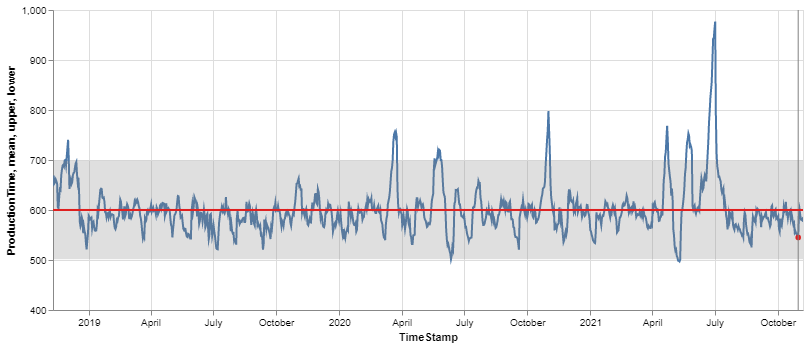
\includegraphics[scale=0.5]{ProductionTime.png}
    \caption{Block Production Time}
\end{figure}
Through the bar chart, it looks like that the production time follows a normal distribution. The distribution is skewed a bit due to the outliers.  
\begin{figure}[H]
    \centering
    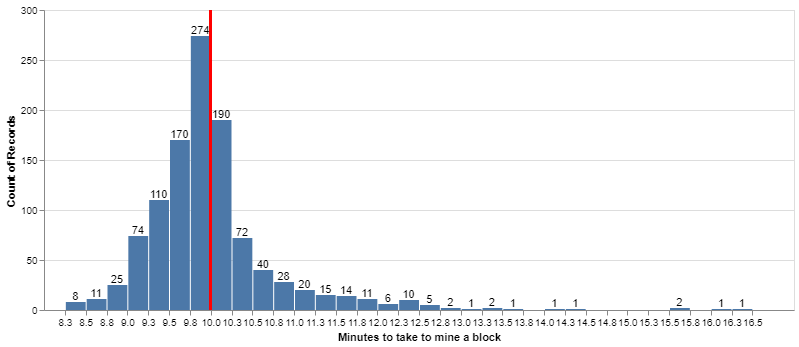
\includegraphics[scale=0.5]{ProductionTimeDistribution.png}
    \caption{Distribution of Block Production Time}
\end{figure}
As for the transaction fee, there is no obvious pattern in it. What's more, its volatility is so big that its standard deviation is even larger than the average. 
\begin{table}[H]
    \centering
    \begin{tabular}{@{}|c|c|@{}}
    \hline
    Indicator   & Average Transaction Fee(dollars)  \\ \hline
    mean        & 4.65   \\ \hline
    std         & 7.5   \\ \hline
    min         & 0.14   \\ \hline
    median      & 2.03   \\ \hline
    max         & 74.78   \\ \hline
    \end{tabular}
\end{table}
\begin{verbatim}
    transaction_df["dow"] = pd.to_datetime(df.index).dayofweek
    model = smf.ols(data=transaction_df, formula="AverageTransactionFee ~ C(dow)").fit()
    transaction_df["AverageTransactionFee_ds"] = model.resid + \
    transaction_df["AverageTransactionFee"].mean()
    transaction_df = transaction_df.melt(id_vars="TimeStamp", \
    value_vars=["AverageTransactionFee", "AverageTransactionFee_ds"])
\end{verbatim}
\par The high transaction fee must be a disadvantage of bitcoin. In addition, although there is a lot of vibration within the transaction fee, it turns out there is no seasonal effect in it. To dig out more information about the transaction fee, we'll find more relationships between it and other variables in question 2.
\begin{figure}[H]
    \centering
    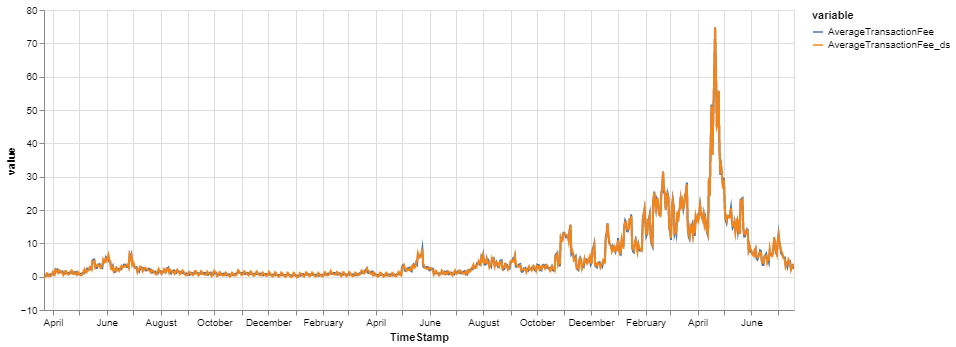
\includegraphics[scale=0.5]{AverageTransactionFee.png}
    \caption{Transaction Fee}
\end{figure}
\subsection{Question 2}
\begin{verbatim}
    data = df[["CloseBTC", "MinerRevenue", "UniqueAddress", "Transactions", \
    "TransactionFee", "TotalHashRate"]].copy()
    data["AverageTransactionFee"] = data["TransactionFee"] / data["Transactions"]
    data["HashRevenue"] = data["MinerRevenue"] / data["TotalHashRate"]
    del data["TransactionFee"], data["TotalHashRate"]
    corr = data.corr().reset_index().melt(
        id_vars=["index"], 
        value_vars=["CloseBTC", "MinerRevenue", "UniqueAddress", "Transactions",\
        "AverageTransactionFee", "HashRevenue"],
        value_name="coeff"
    ).rename(columns={"index": "field1", "variable":"field2"})
\end{verbatim}
\par After doing the preprocessing, I calculate the correlation matrix of different fields and plot the heatmap. The heatmap shows that there is a significant linear relationship between miner revenue and the close price. It must be because the revenue of miners is calculated in Bitcoins, and higher bitcoin prices will encourage more people to invest in mining. A similar idea also applied to the average transaction fee. Since the fee is also calculated in Bitcoins, it will also increase when Bitcoin's price goes up.
\begin{figure}[H]
    \centering
    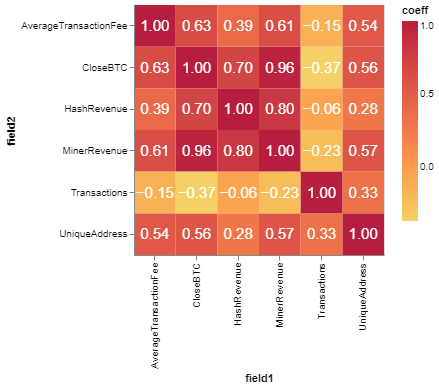
\includegraphics[scale=0.5]{Heatmap.png}
    \caption{Heatmap of correlation Matrix}
\end{figure}
Then I performed Z-score normalization and 7-day window smoothing on each variable, and it looks that there are a lot of moments where variables behave in a similar pattern.
\begin{figure}[H]
    \centering
    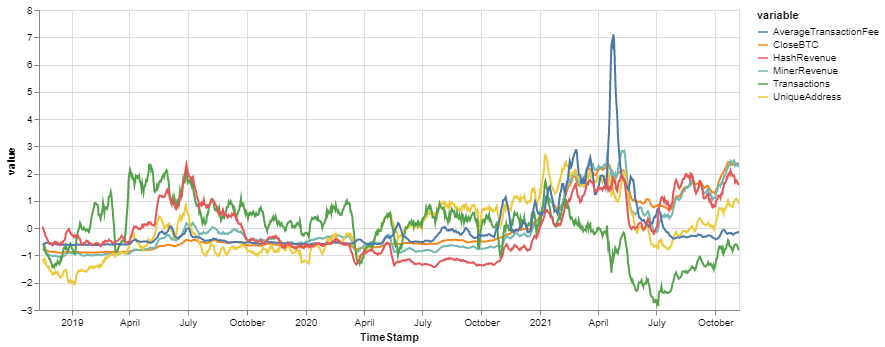
\includegraphics[scale=0.5]{LineChart.png}
    \caption{Line chart of Z-scored smooth variables}
\end{figure}
\begin{verbatim}
    for column in diff_data.columns:
        diff_data[column] = diff_data[column] / diff_data[column].shift(1)
    corr_diff = diff_data.corr().reset_index().melt(
        id_vars=["index"], 
        value_vars=["CloseBTC", "MinerRevenue", "UniqueAddress", "Transactions",\
        "AverageTransactionFee", "HashRevenue"],
        value_name="coeff"
    ).rename(columns={"index": "field1", "variable":"field2"})
\end{verbatim}
By calculating the correlation of the difference of each field, I find another significant relationship between the transaction and unique address, which means these two variables usually behave similarly in a short period.
\begin{figure}[H]
    \centering
    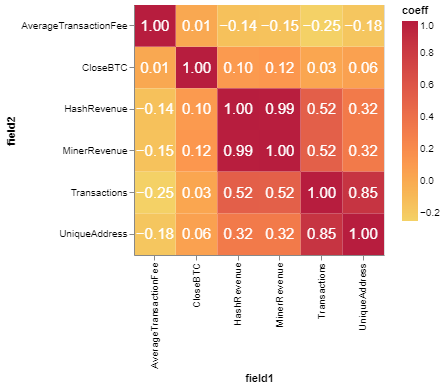
\includegraphics[scale=0.5]{HeatmapDiff.png}
    \caption{Heatmap of correlation Matrix of Percentage Difference}
\end{figure}
\par After carefully reviewing the line chart, I think the result is correct. Although there is no clear linear relationship between transactions and unique addresses, they do behave in the same way frequently. In addition, I also find there is a relationship between the miner's revenue and the number of transactions. When the number of transactions rises or drops quickly, the miner's revenue will behave in the same way too.
\begin{figure}[H]
    \centering
    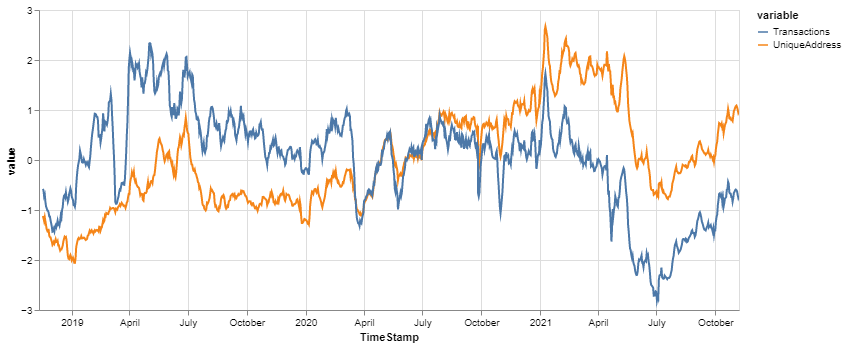
\includegraphics[scale=0.5]{TransactionAddress.png}
    \caption{Line chart of Z-scored smooth variables}
\end{figure}
\subsection{Question 3}
\begin{verbatim}
    BTC_df = df[["CloseBTC", "TradeCountBTC", "TradeVolumeBTC", "Transactions", "Difficulty", \
    "UniqueAddress"]].copy()
    ETH_df = df[["CloseETH", "TradeCountETH", "TradeVolumeETH"]].copy()
    BTC_df["ReturnBTC"] = BTC_df["CloseBTC"].shift(-1) / BTC_df["CloseBTC"]
    ETH_df["ReturnETH"] = ETH_df["CloseETH"].shift(-1) / ETH_df["CloseETH"]
    def PCA():
        BTC_PCA_df = BTC_df.copy()
        for column in BTC_PCA_df.columns:
            BTC_PCA_df[column] = BTC_PCA_df[column].rolling(window=7).mean()
        BTC_PCA_df = BTC_PCA_df.dropna()
        for column in BTC_PCA_df.columns:
            BTC_PCA_df[column] = max(BTC_PCA_df[column]) - BTC_PCA_df[column]
            BTC_PCA_df[column] = (BTC_PCA_df[column] - BTC_PCA_df[column].mean()) / \
            BTC_PCA_df[column].std()
        
        pca_model = skd.PCA().fit(BTC_PCA_df)
        X = pca_model.transform(BTC_PCA_df)
        plt.figure(figsize=(8,6))
        plt.scatter(X[:,0], X[:,1])
        plt.xlabel('PC1')
        plt.ylabel('PC2')
        plt.title('BTC BiPlot')
        plt.xlim(-6, 6)
        plt.ylim(-10, 4)
        # Add variable unit vector projections
        V = pca_model.transform(np.identity(X.shape[1]))
        for i, v in enumerate(V):
            plt.annotate(BTC_df.columns[i], 
                         xy=(0,0), xytext=v[:2]*10, 
                         fontsize=10, color='orange',
                         arrowprops=dict(
                            arrowstyle='<-', linewidth=2, color='orange'))
        plt.savefig("./BTCBiPlot.png")
        return plt.show()
    PCA()
\end{verbatim}
Firstly, I performed PCA to reduce the dimension of the BTC's data, and it turns out that the difficulty, trade count, and total trade volume are very correlated to each other. On the other hand, there is no variable close to the return, meaning that we need more information to make a stable profit through cryptocurrencies.
\begin{figure}[H]
    \centering
    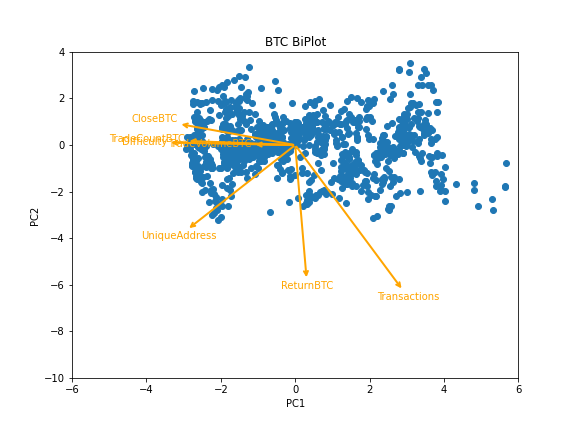
\includegraphics[scale=0.5]{BTCBiPlot.png}
    \caption{BTC Biplot}
\end{figure}
\begin{verbatim}
    invest = pd.DataFrame(columns=["Cash","ETH", "BTC"])
    ETH, BTC = 0, 0
    Cash = 156
    for i in range(0, len(BTC_df), 7):
        Cash -= 1
        ETH += 1 / ETH_df.iloc[i]["CloseETH"]
        BTC += 1 / BTC_df.iloc[i]["CloseBTC"]
        invest.loc[BTC_df.iloc[i].name] = [Cash, ETH, BTC]
    invest["InvestETH"], invest["InvestBTC"] = ETH_df["CloseETH"], BTC_df["CloseBTC"]
    invest["StrategyETH"] = invest["Cash"] + invest["ETH"] * invest["InvestETH"]
    invest["StrategyBTC"] = invest["Cash"] + invest["BTC"] * invest["InvestBTC"]
    invest["StrategyETH"] = invest["StrategyETH"] / 156 
    invest["StrategyBTC"] = invest["StrategyBTC"] / 156 
    invest["InvestETH"] = invest["InvestETH"] / invest["InvestETH"].iloc[0] 
    invest["InvestBTC"] = invest["InvestBTC"] / invest["InvestBTC"].iloc[0]
    invest["InvestHash"] = (df["MinerRevenue"] / df["TotalHashRate"]).cumsum() * 13.5 / 800 + 1
    data = invest[["InvestETH", "InvestBTC", "StrategyETH", "StrategyBTC", "InvestHash"]].\(\)reset_index().rename(columns={"index":"TimeStamp"}).melt(id_vars=["TimeStamp"])
\end{verbatim}
Then, I simulate the investment process of cryptocurrencies. The strategies include buying and hold and investing a specific amount of money every week, and the assets include ETH and BTC. In addition, I also calculate the hash rate revenue to simulate the miner's investment. According to the result, it turns out that investing in ETH will lead to a much higher profit than bitcoin. What's more, the weekly investment strategy will always lead to higher revenue than buy and hold, even though there's a revenue chart that has a similar pattern.
As for the miners, their profit is more stable, and they will always make more profit until 2021. Therefore, the golden age for miners has already passed, but it's still a good choice for people who hate loss.
\begin{figure}[H]
    \centering
    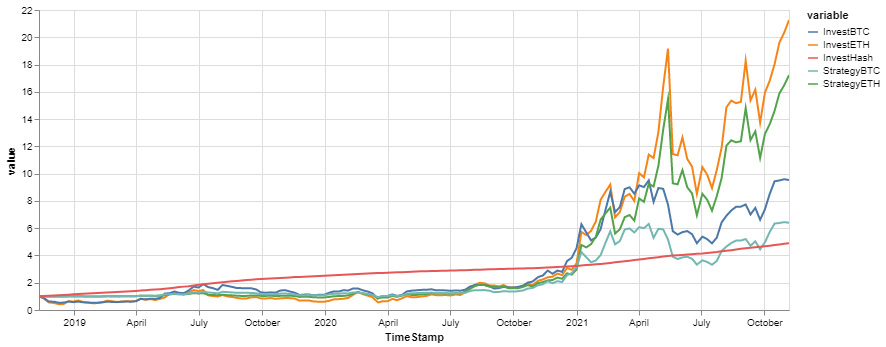
\includegraphics[scale=0.5]{Investment.png}
    \caption{Invest Revenue of cryptocurrencies}
\end{figure}
\section{Conclusion}
Based on my analysis and visualization, I can answer the previous questions
\begin{enumerate}[1]
    \item Does Bitcoin work as it is supposed to? \\ Bitcoin does an excellent job at adjusting the network difficulty based on the total hash rate. The production time for each block is never smaller than 490 seconds and has an average value of 600 seconds, as stated in the white paper. What's more, I guessed that the high peak in the production time is due to the shut down of the big miner field. For the transaction fee, as what Bitcoin is criticized for, the fee is high and volatile.
    \item How are people's activities on Bitcoin’s blockchain? \\ The user number of Bitcoin is a wide range, from 300k to 1m. What's more, there is a significant relationship between the number of users and the number of transactions. Usually, they will have the same rise or drop. As for the miner's revenue, it's typically determined by the price of Bitcoin, and it's because the revenue is calculated in Bitcoin. What's more, through the correlation matrix of percentage difference, I also find that sometimes the revenue will behave in the same way as the transaction. Chances are that when there are more transactions, the award in each block is higher, so the revenue is higher too.
    \item Can we make profit through cryptocurrencies investment? \\ The result shows that there is no significant relationship between the return and other variables, while difficulty, trading volume, and trading counts are very similar. To make an accurate prediction for the cryptocurrencies' price, we need a better model and much more kinds of data. However, a simple way to make a profit through cryptocurrencies is to invest a specific amount of money into ETH periodically. For people who hate loss, investing money to be a miner will be a better choice because it can provide a stable revenue without any drawback.
\end{enumerate}
\end{document}